\def\tenchude{ỨNG DỤNG THỰC TẾ}
\section{Ứng dụng đạo hàm và khảo sát hàm số để giải quyết một số bài toán thực tiễn}
\subsection{Lý thuyết cần nhớ}
\subsubsection{Tốc độ thay đổi của một đại lượng}
Ta có đạo hàm $f'(a)$ là tốc độ thay đổi tức thời của đại lượng $y=f(x)$ đối với $x$ tại điểm $x=a$. Dưới đây, chúng ta xem xét một số ứng dụng của ý tưởng này đối với vật lí, hoá học, sinh học và kinh tế: 
\begin{itemize}
	\item Nếu $s=s(t)$ là hàm vị trí của một vật chuyển động trên một đường thẳng thì $v=s'(t)$ biểu thị vận tốc tức thời của vật (tốc độ thay đổi của độ dịch chuyển theo thời gian). Tốc độ thay đổi tức thời của vận tốc theo thời gian là gia tốc tức thời của vật:
	$$
	a(t)=v'(t)=s''(t).
	$$
	\item Nếu $C=C(t)$ là nồng độ của một chất tham gia phản ứng hoá học tại thời điểm $t$, thì $C'(t)$ là tốc độ phản ứng tức thời (tức là độ thay đổi nồng độ) của chất đó tại thời điểm $t$.
	\item Nếu $P=P(t)$ là số lượng cá thể trong một quần thể động vật hoặc thực vật tại thời điểm $t$, thì $P'(t)$ biểu thị tốc độ tăng trưởng tức thời của quần thể tại thời điểm $t$.
	\item  Nếu $C=C(x)$ là hàm chi phí, tức là tổng chi phí khi sản xuất $x$ đơn vị hàng hoá, thì tốc độ thay đổi tức thời $C'(x)$ của chi phí đối với số lượng đơn vị hàng được sản xuất được gọi là chi phí biên.
	\item Về ý nghĩa kinh tế, chi phí biên $C'(x)$ xấp xỉ với chi phí để sản xuất thêm một đơn vị hàng hoá tiếp theo, tức là đơn vị hàng hoá thứ $x+1$ (xem SGK Toán 11 tập hai, trang 87, bộ sách Kết nối tri thức với cuộc sống). 
\end{itemize}
\subsubsection{Bài toán tối ưu hóa}
Một trong những ứng dụng phổ biến nhất của đạo hàm là cung cấp một phương pháp tổng quát, hiệu quả để giải những bài toán tối ưu hoá. Trong mục này, chúng ta sẽ giải quyết những vấn đề thường gặp như tối đa hoá diện tích, khối lượng, lợi nhuận, cũng như tối thiểu hoá khoảng cách, thời gian, chi phí. Quy trình giải một số bài toán tối ưu hoá  đơn giản:
% \begin{gachsoc}
	\begin{itemize}
		\item[\iconCH]\indamm{Bước 1.} Xác định đại lượng Q mà ta cần làm cho giá trị của đại lượng ấy lớn nhất hoặc nhỏ nhất và biểu diễn nó qua các đại lượng khác trong bài toán.
		
		\item[\iconCH]\indamm{Bước 2.}  Chọn một đại lượng thích hợp nào đó, kí hiệu là $x$, và biểu diễn các đại lượng khác ở \indamm{Bước 1} theo $x$. Khi đó, đại lượng $Q$ sẽ là hàm số của một biến $x$. Tìm tập xác định của hàm số $Q=Q(x)$.
		
		\item[\iconCH]\indamm{Bước 3.}  Tìm giá trị lớn nhât hoặc giá trị nhỏ nhất của hàm số $Q=Q(x)$ bằng các phương pháp đã biết và kết luận.
	\end{itemize}
% \end{gachsoc}
\subsection{Phân loại và phương pháp giải toán}
% \boxmini{BÀI TẬP TỰ LUẬN}
\begin{dang}{Bài toán về quãng đường, vận tốc, gia tốc}
	\begin{listEX}[1]
		\item [\ding{172}] Nếu phương trình chuyển động của vật là $s=f(t)$ thì $v=f^{\prime}(t)$ là vận tốc tức thời và $a=v^{\prime}(t)$ là gia tốc tức thời của vật tại thời điểm $t$.
		\item [\ding{173}] Trong chuyển động thẳng đều thì $s=v \cdot t$.
	\end{listEX}
\end{dang}


\begin{vd}
	Trong $3$ giây đầu tiên, một chất điểm chuyển động theo phương trình $$s(t)=-t^3+6t^2+t+5,$$ trong đó $t$ tính bằng giây và $s$ tính bằng mét. Chất điểm có vận tốc tức thời lớn nhất bằng bao nhiêu trong $3$ giây đầu tiên đó?
	\loigiai{
		Vận tốc tức thời của chất điểm là $v(t)=s'(t)=-3t^2+12t+1$. Ta có
		\begin{itemize}
			\item [] $v'(t)=-6t+12$;
			\item [] $v'(t)=0\Leftrightarrow t=2$.
		\end{itemize}
		Bảng biến thiên của hàm số $v(t)$ trên đoạn $[0;3]$ như sau:
		\begin{center}
			
\begin{tikzpicture}
				\tkzTabInit[nocadre=false,lgt=1.2,espcl=2.5]
				{$t$ /0.6,$v'(t)$ /0.6,$v(t)$ /2}
				{$0$,$2$,$3$}
				\tkzTabLine{,+,$0$,-,}
				\tkzTabVar{-/$1$, +/$13$,-/$10$}
			\end{tikzpicture}
		\end{center}
		Suy ra, vận tốc lớn nhất $v_{\max}=13$ (m/s) khi $t=2$ (s).
	}
\end{vd}
\dongcham{7}
\begin{vd}
	Khi bỏ qua sức cản của không khí, độ cao (mét) của một vật được phóng thẳng đứng lên trên từ điểm cách mặt đất $2$ m với vận tốc ban đầu $24{,}5$ m/s là $h(t)=2+24{,}5t-4{,}9t^2$ (theo Vật lí đại cương, NXB Giáo dục Việt Nam, $2016$).
	\begin{enumerate}
		\item Tìm vận tốc của vật sau $2$ giây.
		\item Khi nào vật đạt độ cao lớn nhất và độ cao lớn nhất đó là bao nhiêu?
		\item Khi nào thì vật chạm đất và vận tốc của vật lúc chạm đất là bao nhiêu?
	\end{enumerate}
	\loigiai{
		\begin{enumerate}
			\item Theo ý nghĩa cơ học của đạo hàm, vận tốc của vật là $v=h'(t)=24{,}5-9{,}8t$ m/s.\\				
			Do đó, vận tốc của vật sau $2$ giây là $v(2)=24{,}5-9{,}8\cdot 2=4{,}9$ m/s.
			\item Vì $h(t)$ là hàm số bậc hai có hệ số $a=-4{,}9< 0$ nên $h(t)$ đạt giá trị lớn nhất tại $t=-\dfrac{b}{2a}=\dfrac{24{,}5}{2\cdot 4{,}9}=2{,}5$ (giây). Khi đó, độ cao lớn nhất của vật là $h(2{,}5)=32{,}625$ m.
			\item Vật chạm đất khi độ cao bằng 0, tức là $h=2+24{,}5t-4{,}9t^2=0$, hay $t \approx 5{,}08$ (giây).\\
			Vận tốc của vật lúc chạm đất là $v(5{,}08)=24{,}5-9{,}8\cdot 5{,}08=-25{,}284$ m/s.\\
			Vận tốc âm chứng tỏ chiều chuyển động của vật là ngược chiều dương (hướng lên trên) của trục đã chọn (khi lập phương trình chuyển động của vật).
		\end{enumerate}
	}
\end{vd}
\dongcham{11}
\begin{vd}
	\immini
	{Anh An chèo thuyền từ điểm $A$ trên bờ một con sông thẳng rộng $3$ km và muốn đến điểm $B$ ở bờ đối diện cách $8$ km về phía hạ lưu càng nhanh càng tốt (hình bên). Anh An chèo thuyền đến một điểm $D$ nào đó giữa $C$ và $B$ rồi chạy bộ đến $B$. Nếu vận tốc chèo thuyền là $6$ km/h và vận tốc chạy bộ là $8$ km/h thì anh An phải chèo thuyền sang bờ ở điểm $D$ cách $B$ bao nhiêu km để đến được $B$ càng sớm càng tốt? (\textit{Giả sử rằng vận tốc của nước là không đáng kể so với vận tốc chèo thuyền của anh An}).}
	{
		\begin{tikzpicture}[>=stealth,scale=0.5]
			\def\d{3}
			\draw (0,2)--(0,-9) (3,2)--(3,-9);
			\path (0,0) coordinate (A)
			(3,0) coordinate (C)
			(3,-\d) coordinate (D)
			(3,-8) coordinate (B);
			\foreach\x/\y in {B/below right,C/above right,D/below right} \draw[->] (A) node[left]{$A$}--(\x) node[\y]{$\x$};
			\draw[<->] ($(C)+(1.2,0)$)--($(B)+(1.2,0)$) node[right,midway]{$8$ km};
			\draw[<->] ($(C)+(0.3,0)$)--($(D)+(0.3,0)$) node[right,midway]{$x$};
			\draw[<->] (0,1)--(3,1) node[above,midway]{$3$km};
			\draw [dashed] (C)--($(C)+(1.5,0)$) (B)--($(B)+(1.5,0)$) (D)--($(D)+(0.5,0)$);
		\end{tikzpicture}
	}
	\loigiai{
		Gọi độ dài đoạn $ CD $ là $ x $ (km), với $0 \leq x \leq 8$. Khi đó 
		\begin{itemize}
			\item [$\bullet$] Độ dài quãng đường $A D$ là $\sqrt{9+x^2}$ và thời gian đi hết quãng đường $ AD $ là $\dfrac{\sqrt{9+x^2}}{6}$;
			\item [$\bullet$] Độ dài quãng đường $ BD $ là $ 8 - x $ và thời gian đi hết quãng đường $ BD $ là $\dfrac{8-x}{8}$.
		\end{itemize}
		Tổng thời gian người đó đi từ $A$ đến $B$ là 
		$$f(x)=\dfrac{\sqrt{9+x^2}}{6}+\dfrac{8-x}{8}\quad (h)$$
		Ta có
		\begin{itemize}
			\item [$\bullet$] $f'(x)=\dfrac{x}{6 \sqrt{9+x^2}}-\dfrac{1}{8}$;
			\item [$\bullet$] $f'(x)=0 \Leftrightarrow \dfrac{x}{6 \sqrt{9+x^2}}-\dfrac{1}{8}=0$\\
			\hspace*{1.7cm} $\Leftrightarrow 8 x=6 \sqrt{9+x^2} \Leftrightarrow \heva{&x \geq 0 \\ &64 x^2=36\left(9+x^2\right)} \Leftrightarrow x=\dfrac{9 \sqrt{7}}{7}$.
		\end{itemize}
		Bảng biến thiên của hàm số $f(x)$ trên $[0;8]$ như sau:
		\begin{center}
			
\begin{tikzpicture}[font=\footnotesize,thick,>=stealth]
				\tikzset{double style/.append style={double distance=1.5pt}}\tkzTabInit[nocadre=false,lgt=1.2,espcl=3.5,deltacl=0.6,lw=.75pt]
				{$x$ /1.2, $f'(x)$ /0.8, $f(x)$ /2.2}
				{$0$,$\dfrac{9 \sqrt{7}}{7}$,$8$}
				\tkzTabLine{ ,-,$0$,+, }
				\tkzTabVar{+/$\dfrac{3}{2}$,-/$1+\dfrac{\sqrt{7}}{8}$,+/$\dfrac{\sqrt{73}}{6}$}
			\end{tikzpicture}
		\end{center}
		Dựa vào bảng biến thiên ta thấy để đến $B$ sớm nhất thì anh An phải chèo thuyền đến điểm $D$ cách $B$ một đoạn $8-x=8-\dfrac{9 \sqrt{7}}{7}=$ (km).
	}
\end{vd}
\dongcham{12}
\begin{vd}
	Chi phí về nhiên liệu của một con tàu được chia làm hai phần. Phần chi phí thứ nhất không phụ thuộc vào tốc độ tàu và bằng $480 \mathrm{nghìn}$ đồng mỗi giờ. Chi phí phần thứ hai trên 1 km đường tỉ lệ thuận với lập phương của tốc độ tàu, khi tốc độ bằng $20 \mathrm{~km} / \mathrm{h}$ thì chi phí phần thứ hai bằng 100 nghìn đồng mỗi giờ. Giả sử con tàu đó luôn giữ nguyên tốc độ di chuyển, để tổng chi phí nhiên liệu trên 1 km đường là nhỏ nhất thì tốc độ của con tàu đó bằng bao nhiêu $\mathrm{km} / \mathrm{h}$ ?
	\loigiai{
		Gọi $x(\mathrm{~km} / \mathrm{h})$ là tốc độ của tàu. \\
		Thời gian tàu chạy quãng đường 1 km là $\frac{1}{x}$ (giờ).\\
		Chi phí tiền nhiên liệu phần thứ nhất cho quãng đường 1 km là $480 \frac{1}{x}$ (nghìn đồng).\\
		Gọi $y$ (nghìn đồng) là chi phí nhiên liệu phần thứ hai cho quãng đường 1 km ứng với tốc độ $x$.\\
		Ta có $y$ tỉ lệ thuận với lập phương tốc độ nên $y=k x^3$ với $k>0$.\\
		Khi tốc độ $x=20(\mathrm{~km} / \mathrm{h})$ thì thời gian tàu chạy 1 km là $\frac{1}{20}$ (giờ) nên chi phí phần thứ 2 cho quãng đường 1 km là $\frac{1}{20} \cdot 100=5$ (nghìn đồng)\\
		Suy ra $5=k \cdot 20^3$ nên $k=\frac{1}{1600}$, do đó $y=\frac{1}{1600} x^3$\\
		Vậy tổng chi phí tiền nhiên liệu cho 1 km đường là: $P(x)=\frac{480}{x}+\frac{x^3}{1600}$.\\
		Bài toán trở thành tìm $x$ để $P(x)$ nhỏ nhất.\\
		Ta có $P^{\prime}(x)=-\frac{480}{x^2}+\frac{3 x^2}{1600}=0 \Leftrightarrow x=4 \sqrt[4]{1000}$.\\
		Lập bảng biến thiên, suy ra để tổng chi phí trên 1 km đường nhỏ nhất thì vận tốc của tàu là $x=4 \sqrt[4]{1000} \approx 22,5(\mathrm{~km} / \mathrm{h})$.
	}
\end{vd}
\dongcham{13}
\begin{dang}{Bài toán tối ưu hóa trong chi phí, doanh thu, lợi nhuận}
	\begin{itemize}
		\item [\iconCH] Nếu $C(x)$ là tổng chi phí mà công ty (doanh nghiệp) phải trả để sản xuất $x$ đơn vị hàng hóa thì $C(x)$ được gọi là \textbf{hàm chi phí}.
		\item [\iconCH] Gọi $p(x)$ là giá bán mỗi đơn vị hàng hóa khi giao dịch $x$ đơn vị hàng hóa. Khi đó $p(x)$ được gọi là \textbf{hàm cầu} (hay \textbf{hàm giá}) và hàm số này được kì vọng là hàm giảm theo biến $x$.
		\item [\iconCH] Nếu $x$ đơn vị hàng hóa được bán với giá mỗi đơn vị $p(x)$, thì \textbf{hàm doanh thu}, kí hiệu là $R(x)$, được tính bởi công thức $R(x)=x\cdot p(x)$.
		\item [\iconCH] Nếu $x$ đơn vị hàng hóa được bán với giá mỗi đơn vị là $p(x)$, thì \textbf{hàm lợi nhuận}, kí hiệu là $P(x)$, được tính bởi công thức \[P(x)=R(x)-C(x)=xp(x)-C(x).\]
	\end{itemize}
\end{dang}

\begin{vd}
	Tại một xí nghiệp chuyên sản xuất vật liệu xây dựng, nếu trong một ngày xí nghiệp sản xuất $x\, (m^3)$ sản phẩm thì phải bỏ ra các khoản chi phí bao gồm: 5 triệu đồng chi phí cố định; 0,4 triệu đồng chi phí cho mỗi mét khối sản phẩm và $0,005x^2$ triệu đồng chi phí bảo dưỡng máy móc. Biết rằng, mỗi ngày xí nghiệp sản xuất được tối đa 45 $m^3$ sản phẩm.  Tìm chi phí trung bình (triệu đồng) trên mỗi mét khối sản phẩm thấp nhất mà xí nghiệp cần bỏ ra (làm tròn đến hàng phần trăm).
	\loigiai{ 
		
		Tổng chi phí (triệu đồng) để xí nghiệp sản xuất $x (m^3)$ sản phẩm trong một ngày là
		$$C(x)=5+0,4x+0,005x^2, \text{ với }0\le x \le 45.$$
		Chi phí trung bình (triệu đồng) trên mỗi mét khối sản phẩm là		
		$$f(x)=\dfrac{C(x)}{x}=\dfrac{5+0,4x+0,005x^2}{x}=\dfrac{5}{x} + 0,4 + 0,005x.$$
		Ta có
		$$f'(x)=-\dfrac{5}{x^2}+0,005=\dfrac{0,005x^2-5}{x^2}, \quad f'(x)=0 \Rightarrow x^2=1000 \Rightarrow x=\sqrt{1000}.$$
		Bảng biến thiên:
		\begin{center}
			
\begin{tikzpicture}
				\tkzTabInit[espcl=3,lgt=1.5,nocadre=false]
				{$x$/1.2,$f'(x)$/0.7,$f(x)$/2}
				{$0$,$\sqrt{1000}$,$+\infty$}
				\tkzTabLine{d,-,0,+}
				\tkzTabVar{+D+/$ $/$+\infty$,-/$0.72$,+/$+\infty$}
			\end{tikzpicture} 
		\end{center}
		Từ bảng biến thiên ta thấy chi phí trung bình thấp nhất là
		$\overline C(\sqrt{1000})\approx 0,72 $ đạt được khi $x=\sqrt{1000} \approx 32,0$. 
}\end{vd}
\dongcham{9}
\begin{vd}
	Giả sử một loại hàng hoá có hàm cầu được mô hình hoá bởi $ p(x)=100-0{,}5 x $ và hàm chi phí được mô hình hoá bởi $ C(x)=40 x+37{,}5 $, trong đó $ p $ (nghìn đồng) là giá của một đơn vị hàng hoá đó. Hỏi khi lợi nhuận là lớn nhất, chi phí trung bình cho mỗi đơn vị là bao nhiêu nghìn đồng ? (\textit{kết quả làm tròn đến hàng đơn vị}).
	\loigiai{
		Doanh thu của cửa cửa hàng là $R(x)=xp(x)=x(100-0{,}5 x)$.\\
		Lợi nhuận của cửa hàng là 
		$$P(x)=R(x)-C(x)=(100-0{,}5 x)x-(40 x+37{,}5)=-0{,}5x^2+60x-37{,}5$$
		Xét hàm số $P(x)=-0{,}5x^2+60x-37{,}5$, với $x>0$. Ta có
		\begin{itemize}
			\item [$\bullet$] $P^{\prime}(x)=-x+60$;
			\item [$\bullet$] $P^{\prime}(x)=0 \Leftrightarrow -x+60=0 \Leftrightarrow x=60$.
		\end{itemize}
		Bảng biến thiên của hàm $P(x)$:
		\begin{center}
			
\begin{tikzpicture}
				\tkzTabInit
				[lgt=1.5,espcl=4] % tùy chọn
				{$x$/0.6, $P'(x)$/0.6, $P(x)$/2} % cột đầu tiên
				{$0$, $60$, $+\infty$} % hàng 1 cột 2
				\tkzTabLine{,+,0,-,} % hàng 2 cột 2
				\tkzTabVar{-/ , +/ $70$ , -/ } % hàng 3 cột 2
			\end{tikzpicture}
		\end{center}
		Ta thấy, lợi nhuận lớn nhất khi $x=70$. Khi đó, chi phí trung bình là 
		$$\dfrac{C(x)}{x}=\dfrac{40\cdot60+37{,}5}{60}=40{,}625 \approx 41 \text{ (nghìn đồng).}$$
	}
\end{vd}
\dongcham{9}
\begin{vd}%[BG10-2022]%[Toanvo]%[0D4G4-4]
	Một công ty sản xuất và bán hết $x$ sản phẩm $(0<x \leq 1000)$, tổng số tiền công ty thu được là $f(x)=1000 x-x^2$ (nghìn đồng), chi phí sản xuất bình quân cho một sản phẩm là $g(x)=x+\dfrac{30}{x}+680$ (nghìn đồng). Giả sử mức thuế phụ thu trên một đơn vị sản phẩm bán được là $t$ (nghìn đồng) ( $0<t<200$ ). Tìm mức thuế phụ thu $t$ (nghìn đồng) trên một sản phẩm sao cho nhà nước nhận được số tiển thuế phụ thu lớn nhất và công ty cũng thu được lợi nhuận lởn nhất theo mức thuế phụ thu đó.
\end{vd} 
\dongcham{9}
\begin{dang}{Bài toán tối ưu hoá trong hình học}
	\begin{listEX}[1]
		\item [\ding{172}] Thể tích khối hộp chữ nhật $V= \text{ dài } \times \text{ rộng } \times  \text{ cao}$;
		\item [\ding{173}] Thể tích khối lập phương $V= \text{(cạnh)}^3$;
		\item [\ding{174}] Thể tích khối chóp $V= \dfrac{1}{3} \times S_{\text{ đáy}} \times \text{ cao}$;
		\item [\ding{175}] Khối nón:
		\begin{itemize}
			\item [$\bullet$] Diện tích xung quanh: $S_{\text{xq}}=\pi r l$.
			\item [$\bullet$] Thể tích: $V= \dfrac{1}{3} \pi r^2h$.
		\end{itemize}
		\item [\ding{176}] Khối trụ:
		\begin{itemize}
			\item [$\bullet$] Diện tích xung quanh: $S_{\text{xq}}=2\pi r l$.
			\item [$\bullet$] Thể tích: $V= \pi r^2h$.
		\end{itemize}
	\end{listEX}
\end{dang}

\begin{vd}
	\immini{Một bác nông dân có ba tấm lưới B40, mỗi tấm dài $a \text{ (m)}$ và muốn rào một mảnh vườn dọc bờ sông có dạng hình thang cân $ABCD$ như hình bên dưới (bờ sông là đường thẳng $CD$ không phải rào). Hỏi bác đó có thể rào được mảnh vườn có diện tích lớn nhất là bao nhiêu mét vuông?
	}{
\begin{tikzpicture}
	\path 
	(-3,0) coordinate (D)
	(3,0) coordinate (C)
	($(D)+(65:3)$) coordinate (A)
	($(C)+(115:3)$) coordinate (B)
	;
	\fill[cyan!50] (-4.5,-1) rectangle (4,0);
	\draw[thick] (A)--node[above]{$a \text{(m)}$}(B)--node[right]{$a \text{(m)}$}(C)--(D)--node[left]{$a \text{(m)}$} cycle;
	\foreach \x/\g in {A/120,B/60,C/-60,D/-120}		\fill[black] 	(\x) circle (1pt)
	($(\g:3mm)+(\x)$) node {$\x$};
\end{tikzpicture}}
	\loigiai{
		\begin{center}
			\begin{tikzpicture}
				\path 
				(-3,0) coordinate (D)
				(3,0) coordinate (C)
				($(D)+(65:3)$) coordinate (A)
				($(C)+(115:3)$) coordinate (B)
				($(C)!(A)!(D)$) coordinate (M)
				($(C)!(B)!(D)$) coordinate (N)
				;
				\draw[thick] (A)--(B)--(C)--(D)-- cycle;
				\draw[dashed] (A)--(M) (B)--(N);
				\foreach \x/\g in {A/120,B/60,C/-60,D/-120,M/-90,N/-90}		\fill[black] 	(\x) circle (1pt)
				($(\g:3mm)+(\x)$) node {$\x$};
			\end{tikzpicture}
		\end{center}
		Gọi $M$, $N$ lần lượt là hình chiếu vuông góc của $A$, $B$ trên $CD$.\\
		Đặt $x=MD$, $\left( 0<x<a\right)$. Suy ra $AM=\sqrt{AD^2-MD^2}=\sqrt{a^2-x^2}$.\\
		Diện tích của mảnh vườn hình thang cân là $S(x)=\dfrac{(AB+CD)AM}{2}=(a+x)\sqrt{a^2-x^2}$.\\
		Xét hàm số $f(x)= (a+x)\sqrt{a^2-x^2}$ trên khoảng $\left( 0<x<a\right)$.\\
		$f^\prime (x)=\dfrac{-2x^2-ax+a^2}{\sqrt{a^2-x^2}}$, $f^\prime (x)=0\Leftrightarrow \dfrac{-2x^2-ax+a^2}{\sqrt{a^2-x^2}}=0\Leftrightarrow \hoac{&x=-a \notin \left( 0<x<a\right) \\&x=\dfrac{a}{2}\in \left( 0<x<a\right) }$.\\
		Bảng biến thiên hàm số $f(x)$ trên khoảng $\left( 0;a\right)$.
		\begin{center}
			
\begin{tikzpicture}
				\tkzTabInit[lgt=1.2,espcl=4.5,deltacl=0.6]
				{$x$/1,$f'(x)$/1,$f(x)$/3} {$0$,$\dfrac{a}{2}$,$a$}
				\tkzTabLine{,+,0,-,}
				\tkzTabVar{-/$a^2$,+/$\dfrac{3\sqrt{3}a^2}{4}$,-/$0$}
			\end{tikzpicture}
		\end{center}
		Từ bảng biến thiên suy ra $\max\limits_{(0;a)} f(x)=f\left(\dfrac{a}{2}\right)=\dfrac{3\sqrt{3}a^2}{4}$.\\
		Vậy bác nông dân có thể rào được mảnh vườn có diện tích lớn nhất $\dfrac{3\sqrt{3}a^2}{4} \text{ m}^2$.
	}
\end{vd}
\dongcham{20}

\begin{vd}
	\immini{
		Một người quan sát đứng tại điểm $P$, cách xa đường đua một đơn vị độ dài. Hai vận động viên xuất phát từ điểm $S$ và chạy dọc đường đua (như hình vẽ). Biết vận động viên thứ nhất chạy nhanh gấp ba lần vận động viên thứ hai, hãy tìm góc quan sát $\theta$ lớn nhất giữa hai vận động viên mà người quan sát đứng ở $P$ nhìn thấy được.
	}{
		\begin{tikzpicture}[>=stealth]
			\path
			(0,0) coordinate (S)
			(0,3) coordinate (P)
			(4,0) coordinate (M)
			(1.3,0) coordinate (N)
			;
			\draw 
			(P) node[left]{$P$}--(S) node[left]{$S$} node[pos=.5,left]{$1$}
			--(N) node[pos=.5,above]{$t$}--(M)--(P)--(N)
			pic["$\theta$",angle radius=1.75cm]{angle=N--P--M}
			pic["$\psi$",angle radius=2cm]{angle=S--P--N}
			;
			\draw[|<->|] (0,-.5)--(4,-.5) node[pos=.5,fill=white]{$3t$};
		\end{tikzpicture}
	}
	\loigiai{
		Vì góc quan sát $\theta$ có tính chất $0<\theta<\frac{\pi}{2}$ nên việc tìm góc $\theta$ lớn nhất tương đương với việc tìm góc $\theta$ để $\tan\theta$ lớn nhất. Vì vận động viên thứ nhất chạy nhanh gấp $3$ lần vận động viên thứ hai nên khi vận động viên thứ hai cách $S$ một khoảng bằng $t$ thì vận động viên thứ nhất cách $S$ một khoảng là $3t$. Giả sử ta có góc tạo bởi giữa tia $PS$ và hướng từ mắt người quan sát đến người thứ hai là $\psi$ (như hình vẽ), khi đó ta có
		
		$\frac{3t}{1}=\tan(\psi +\theta)=\frac{\tan\psi +\tan\theta}{1-\tan\psi\tan\theta}=\frac{t+\tan\theta}{1-t\tan\theta}\Leftrightarrow \tan\theta=\frac{2t}{1+3t^{2}}$.
		
		Đặt $f(t)=\tan\theta=\frac{2t}{1+3t^{2}}$ thì $f'(t)=\frac{2(1+3t^{2})-12t^{2}}{(1+3t^{2})^{2}}=\frac{2(1-3t^{2})}{(1+3t^{2})}$.
		
		Do vậy $f'(t)=0\Leftrightarrow t=\frac{1}{\sqrt{3}}$ (do $t>0$). Vì $f'(t)$ đổi dấu từ dương sang âm tại $t=\frac{1}{\sqrt{3}}$ nên $f(t)$ đạt giá trị lớn nhất tại $t=\frac{1}{\sqrt{3}}$. Khi đó $\tan\theta=\frac{2\cdot\frac{1}{\sqrt{3}}}{1+3\cdot\frac{1}{3}}=\frac{1}{\sqrt{3}}\Rightarrow\theta=\frac{\pi}{6}$.
		
		Vậy góc quan sát $\theta$ lớn nhất giữa hai vận động viên mà người quan sát đứng ở $P$ nhìn thấy được là $\theta=\frac{\pi}{6}$.\\
		Trong trường hợp này, từ $3t=\tan (\psi+\theta)\Rightarrow\tan\left(\psi+\frac{\pi}{6}\right)\Rightarrow \psi=\frac{\pi}{6}$. Điều này có nghĩa là góc quan sát giữa điểm xuất phát và vận động viên thứ hai của người quan sát đứng ở $P$ cũng là $\frac{\pi}{6}$.
	}
\end{vd}
\dongcham{12}
\begin{vd}%[Đề khảo sát lớp 12 lần 1, 2017 - 2018 trường THPT Cổ Loa, Hà Nội]%[2H1T3]
	\immini{Ông Bình đặt thợ làm một bể cá, nguyên liệu bằng kính trong suốt, không có nắp đậy dạng hình hộp chữ nhật có thể tích chứa được $220500$ cm$^3$ nước. Biết tỉ lệ giữa chiều cao và chiều rộng của bể bằng $3$. Xác định diện tích đáy của bể cá (tính bằng $cm^2$) để tiết kiệm được nguyên vật liệu nhất.
	}{
\begin{tikzpicture}[scale=0.8, font=\footnotesize, line join=round, line cap=round]
	\foreach \x\y\t in {0/0/A,-1/-1.1/B,2.6/-1.1/C}
	\coordinate (\t) at (\x,\y);
	\coordinate (D) at ($(A)+(C)-(B)$);
	\coordinate (A') at ($(A)+(0,3.2)$);
	\coordinate (B') at ($(B)+(0,3.2)$);
	\coordinate (C') at ($(C)+(0,3.2)$);
	\coordinate (D') at ($(D)+(0,3.2)$);
	\draw (B')--(A')--(D')--(C')--(B')--(B)--(C)--(D)--(D')node[midway,right,scale=1]{$h$} (C')--(C);
	\draw[dashed](B)--(A)--(D)node[midway,above,scale=1]{$x$} (A)--(A');
	%\foreach \t/\g in {A/170,B/-150,C/-100,D/0,A'/100,B'/170,C'/-20,D'/50}
	%	\draw[fill=black] (\t) circle(1pt)node[shift={(\g:7pt)}]{$\t$};
\end{tikzpicture}}
	\loigiai{
		Gọi chiều rộng, chiều dài, chiều cao của bể cá lần lượt là $a,b,c$. Ta có $c=3a$ và $b\ge a$.\\
		Thể tích của bể cá là $V=abc=3a^2b=220500$ cm$^3$ $\Leftrightarrow b=\dfrac{73500}{a^2}$.\\
		Vì $a\le b$ và $a\le c$ nên $a^3\le 220500 \Rightarrow a<61$.\\
		Nguyên vật liệu tiết kiệm nhất khi diện tích toàn phần nhỏ nhất.\\
		$S_{tp}=6a^2+\dfrac{514500}{a}$ và  $S'_{tp}=12a-\dfrac{514500}{a^2}=0\Leftrightarrow a=35$.\\
		Bảng biến thiên của $S_{tp}$ là
		\begin{center}
			
\begin{tikzpicture}
				\tkzTabInit[espcl=2.2]
				{$a$/0.7,$S'_{tp}$/0.8, $S_{tp}$/2}
				{$0$, $35$, $61$}
				\tkzTabLine{,-,0,+,}
				\tkzTabVar{+/,-/,+/}
			\end{tikzpicture}
		\end{center}
		Do đó diện tích toàn phần nhỏ nhất khi $a=35$.\\
		Diện tích đáy $S=ab=\dfrac{73500}{a}=2100$ cm$^2$.
	}
\end{vd}
\dongcham{14}
\begin{vd}
	\immini{Khi sản xuất vỏ lon sữa bò hình trụ, các nhà thiết kế luôn đặt mục tiêu sao cho chi phí nguyên liệu làm vỏ lon là ít nhất, tức là diện tích toàn phần của hình trụ là nhỏ nhất. Muốn thể tích khối trụ đó bằng $1 \textrm{ dm}^3$ và diện tích toàn phần của hình trụ nhỏ nhất thì bán kính đáy của hình trụ phải bằng bao nhiêu dm? (\textit{kết quả làm tròn đến hàng phần trăm}).}{
		\begin{tikzpicture}[line join=round,line cap=round,line width=.6pt,font=\footnotesize,scale=0.45,>=stealth]
			\coordinate[label=right:$A$] (A) at (3,0);
			\coordinate[label=left:$O$] (O) at (0,0);
			\coordinate[label=right:$A'$] (A1) at ($(A)+(90:6)$);
			\coordinate[label=left:$O'$] (O1) at ($(O)+(90:6)$);
			\draw (A) arc (0:-180:3 and 3/4)--($(A1)!2!(O1)$) arc (180:0:3 and 3/4) arc (0:-180:3 and 3/4) (A)--(A1)--(O1);
			\draw[dashed] (O1)--(O)--(A) arc (0:180:3 and 3/4);
			\fill (O)circle(1.5pt) (O1)circle(1.5pt) (A)circle(1.5pt) (A1)circle(1.5pt);
	\end{tikzpicture}}
	\loigiai{
		Đổi $1 \text{ lít} =1000 \text{ cm}^3$.
		\\
		Gọi $r( cm )$ là bán kính đáy của hình trụ, $h( cm )$ là chiều cao của hình trụ.
		\\
		Diện tích toàn phần của hinh trụ là $S=2 \pi r^2+2 \pi r h$.
		\\
		Do thể tích của hình trụ là $1000 \text{ cm}^3$ nên ta có: $1000=V=\pi r^2 h$, hay $h=\dfrac{1000}{\pi r^2}$.
		\\
		Do đó, diện tích toàn phần của hình trụ là $S=2 \pi r^2+\dfrac{2000}{r},\, r>0$.
		\\
		Ta cần tìm $r$ sao cho $S$ đạt giá trị nhỏ nhất. Ta có
		\begin{align*}
			&S'=4 \pi r-\dfrac{2000}{r^2}=\dfrac{4 \pi r^3-2000}{r^2};
			\\
			&S'=0 \Leftrightarrow \pi r^3=500 \Leftrightarrow r=\sqrt[3]{\dfrac{500}{\pi}}
		\end{align*}
		Bảng biến thiên
		\begin{center}
			
\begin{tikzpicture}[font=\footnotesize,thick,>=stealth]
				\tikzset{double style/.append style={double distance=1.5pt}}\tkzTabInit[nocadre=false,lgt=1.2,espcl=3.5,deltacl=0.6,lw=.75pt,color,colorL=green!50,colorV=green!50]
				{$r$ /1.2, $S'(r)$ /1, $S(r)$ /2.5}
				{$0$,$\sqrt[3]{\dfrac{500}{\pi}}$,$+\infty$}
				\tkzTabLine{ ,-,$0$,+, }
				\tkzTabVar{+/$+\infty$,-/$S\left( \sqrt[3]{\dfrac{500}{\pi}} \right)$,+/$+\infty$}
			\end{tikzpicture}
		\end{center}
		Khi đó
		$$
		h=\dfrac{1000}{\pi r^2}=\dfrac{1000}{\pi \sqrt[3]{\frac{250000}{\pi^2}}}=\dfrac{100}{\sqrt[3]{250 \pi}}.
		$$
		Vậy cần sản xuất các hộp đựng hình trụ có bán kinh đáy $r=\sqrt[3]{\dfrac{500}{\pi}} \approx 5,42 \text{ (cm)}$ và chiều cao $h=\dfrac{100}{\sqrt[3]{250 \pi}} \approx 10,84\text{ (cm)}$.
	}
\end{vd}
\dongcham{13}

\begin{dang}{Bài toán về tốc độ thay đổi của một đại lượng}
\end{dang}

\begin{vd}
	Khi máu di chuyển từ tim qua các động mạch chính rồi đến các mao mạch và quay trở lại qua các tĩnh mạch, huyết áp tâm thu (tức là áp lực của máu lên động mạch khi tim co bóp) liên tục giảm xuống. Giả sử một người có huyết áp tâm thu $P$ (tính bằng mmHg) được cho bởi hàm số
	$$
	P(t)=\dfrac{25 t^2+125}{t^2+1}, 0 \leq t \leq 10,
	$$
	trong đó thời gian $t$ được tính bằng giây. Tính tốc độ thay đổi của huyết áp sau $5$ giây kể từ khi máu rời tim.
	\loigiai{
		Ta có tốc độ thay đổi của huyết áp là $P'(t)=\dfrac{-100t}{(t^2+1)^2}$. 	Do đó tốc độ thay đổi huyết áp sau $5$ s là $P'(5)=-\dfrac{125}{169}$.
	}
\end{vd}
\dongcham{13}
\begin{vd}
	Doanh số bán hệ thống âm thanh nối mới trong một khoảng thời gian dự kiến sẽ tuân theo đường cong logistic $R=R(x)=\dfrac{5000}{1+5 e^{-x}}, x \geq 0$, trong đó thời gian $x$ được tính bằng năm. Hỏi tốc độ bán hàng đạt tới đa vào năm nào?
	\loigiai{
		Hàm biểu thị tốc độ bán hàng là $f(x)=R^{\prime}(x)=\frac{25000 \mathrm{e}^{-x}}{\left(1+5 \mathrm{e}^{-x}\right)^2}$, với $x \geq 0$. Ta có:
		
		$$
		\begin{aligned}
			f'(x) & =\frac{-25000 \mathrm{e}^{-x}\left(1+5 \mathrm{e}^{-x}\right)^2+25000 \mathrm{e}^{-x} \cdot 2\left(1+5 \mathrm{e}^{-x}\right) \cdot 5 \mathrm{e}^{-x}}{\left(1+5 \mathrm{e}^{-x}\right)^4} \\
			& =\frac{25000 \mathrm{e}^{-x}\left(5 \mathrm{e}^{-x}-1\right)}{\left(1+5 \mathrm{e}^{-x}\right)^3} ; \\
			f'(x) & =0 \Leftrightarrow x=\ln 5 \approx 1,61 .
		\end{aligned}
		$$
		Lập bảng biến thiên:
		\begin{center}
			
\begin{tikzpicture}
				\tkzTabInit[nocadre=false,lgt=1,espcl=2.5]
				{$x$ /0.6,$f'(x)$ /0.6,$f(x)$ /2}
				{$0$, $1{,}61$ ,$+\infty$}
				\tkzTabLine{,+,$0$,-,}
				\tkzTabVar{-/, +/,-/}
			\end{tikzpicture}
		\end{center}
		
		Từ bảng biến thiên, ta thấy tốc độ bán hàng đạt tối đa vào thời điểm năm thứ nhất hoặc năm thứ hai.\\
		Ta có $f(1)=1140,8$, $f(2)=1203,5$. Vậy, tốc độ bán hàng đạt tối đa vào thời điểm năm thứ hai.
		
		
		
	}
\end{vd}
\dongcham{14}
\begin{vd}
	Giả sử số lượng của một quần thể nấm men tại môi trường nuôi cấy trong phòng thí nghiệm được mô hình hoá bằng hàm số $P(t)=\dfrac{a}{b+\mathrm{e}^{-0{,}75t}}$, trong đó thời gian $t$ được tính bằng giờ. Tại thời điểm ban đầu $t=0$, quần thể có 20 tế bào và tăng với tốc độ $12$ tế bào/giờ. Tìm các giá trị của $a$ và $b$. Theo mô hình này, điều gì xảy ra với quần thể nấm men về lâu dài?
	\loigiai{
		Ta có $P'(t)=\dfrac{0,75a \mathrm{e}^{-0,75t}}{\left(b+\mathrm{e}^{-0{,}75t}\right)^2}, t \geq 0$.\\
		Theo đề bài, ta có $P(0)=20$ và $P'(0)=12$. Do đó, ta có hệ phương trình:
		$$
		\heva{&\dfrac{a}{b+1}=20 \\& \dfrac{0,75a}{(b+1)^2=12}} \Leftrightarrow \heva{&a=20(b+1)\\&\dfrac{15}{b+1}=12}
		$$
		Giải hệ phương trình này, ta được $a=25$ và $b=\dfrac{1}{4}$.\\
		Khi đó, $P'(t)=\dfrac{18{,}75\mathrm{e}^{-0{,}75t}}{\left(\dfrac{1}{4}+\mathrm{e}^{-0{,}75 t}\right)^2} > 0, \forall t \geq 0$, tức là số lượng quần thể nấm men luôn tăng.\\
		Tuy nhiên, do $\lim\limits_{t \rightarrow+\infty} P(t)=\lim\limits_{t \rightarrow+\infty} \dfrac{25}{\dfrac{1}{4}+\mathrm{e}^{-0{,}75t}}=100$ nên số lượng quần thể nấm men tăng nhưng không vượt quá $100$ tế bào. 
	}
\end{vd}
\dongcham{10}
\begin{vd}
	
	\immini{Một bể nước có dạng hình nón ngược với bán kính đáy bằng 2 m và chiều cao bằng 4 m (tham khảo hình vẽ dưới đây). Nước được bơm vào bể với tốc độ không đổi là $2 \mathrm{~m}^3 / \mathrm{phút}$. Hỏi tốc độ dâng lên của mực nước (đơn vị $\mathrm{m} / \mathrm{phút}$ ) bằng bao nhiêu khi mực nước trong bể đạt độ sâu bằng 3 m (làm tròn kết quả dến hàng phần trăm)?
	}{
	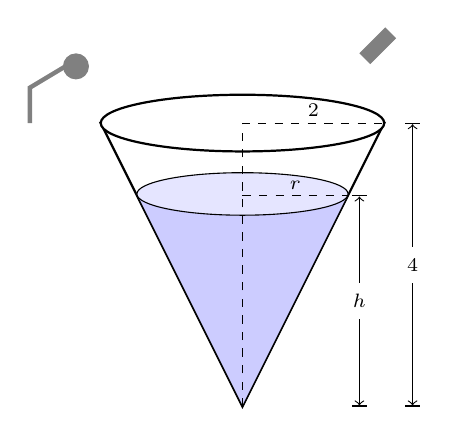
\begin{tikzpicture}[scale=0.9,important line/.style={thick}]
		\draw [opacity=1,important line] (-2,4) -- (2,4) -- (0,0) -- cycle;%big triangle
		\draw [important line,fill=white,opacity=1] (0,4) circle (2cm and 0.4cm);%top of cone
		\draw [fill=blue!20!white,opacity=1] (-1.49,2.98) -- (1.49,2.98) -- (0,0) -- cycle;%smmall triangle
		\draw [fill=blue!10!white,opacity=1,] (0,3) circle (1.49cm and 0.3cm); %top of small cone
		\draw[dashed] (0,0) -- (0,4) --(2,4); %dashed lines
		\draw (1,4.18) node{\scriptsize $ 2 $}; % number
		\draw[dashed] (0,2.98) -- (1.49,2.98); %dashed line
		\draw (0.745,3.12) node{\scriptsize $ r $}; % r
		\draw[|<->|] (2.4,0) -- (2.4,4); %lenght indicator
		\draw[white, fill=white] (2.3,1.75) rectangle (2.5,2.25); %an empty box for the space in middle
		\draw (2.4,2) node{\scriptsize $ 4 $}; %a number
		\draw[|<->|] (1.65,0) -- (1.65,2.98); %lenght indicator
		\draw[white, fill=white] (1.45,1.24) rectangle (1.65,1.74);%white rectangle for a space in middle
		\draw (1.65,1.49) node{\scriptsize $ h $};% h
		\draw[gray,ultra thick] (-3,4) -- (-3,4.5)--(-2.5,4.8); %shower 
		\draw[gray,fill=gray] (-2.35,4.8) circle (5pt); %here the rectangle must join at middle with circle
		\draw[gray,fill=gray,rotate=-45] (-2.35,4.7) rectangle (-2.15,5.2);%bad rectangle, the rotate option moved the rectangle
\end{tikzpicture}}
	\loigiai{
		
	}
\end{vd}
\dongcham{16}
\boxmini{BÀI TẬP TRẮC NGHIỆM}
\ind{PHẦN I.} \inden{Câu trắc nghiệm nhiều phương án lựa chọn.  Mỗi câu hỏi học sinh chỉ chọn một phương án.}\\
\setcounter{ex}{0}
\Opensolutionfile{ans}[ans/2D1-B5-1]

\begin{ex}%[2D1B3-6]%[GHK2 - Thoại Ngọc Hầu - 2018]%[Đỗ Đường Hiếu]%
	Một vật chuyển động theo quy luật $s=-\dfrac{1}{3}t^3+6t^2$ với $t$ (giây) là khoảng thời gian tính từ khi vật bắt đầu chuyển động và $s$ (mét) là quãng đường vật di chuyển được trong khoảng thời gian đó. Hỏi trong khoảng thời gian $7$ giây, kể từ khi bắt đầu chuyển động, vận tốc lớn nhất của vật đạt được bằng bao nhiêu?
	\choice
	{$144$ m/s}
	{$24$ m/s}
	{$180$ m/s}
	{\True $36$ m/s}
	\loigiai{
		Công thức vận tốc chuyển động của vật là $ v(t)=s'(t)=-t^2+12t$.\\
		Ta tìm giá trị lớn nhất của $v(t)$ trên khoảng $(0;7]$.\\
		Ta có $v(t) =36-(t^2-12t+36) =36-\left( t-6 \right)^2 \leq 36$ (m/s).\\
		Do đó $\max\limits_{(0;7]}v(t)=36 \Leftrightarrow t=6$.\\
		Vậy vận tốc lớn nhất của vật trong khoảng thời gian $7$ giây, kể từ khi bắt đầu chuyển động, là $36$ m/s.
	}
\end{ex}
\cham{6}
\begin{ex}
	Một vật chuyền động theo quy luật $s=-\dfrac{1}{2} t^3+6 t^2$ với $t$ (giây) là khoảng thời gian tính từ khi vật bắt đầu chuyển động và $s$ (mét) là quãng đường vật di chuyền được trong khoảng thời gian đó. Hỏi trong khoảng thời gian 9 giây, kể từ khi bắt đầu chuyển động, vận tốc lớn nhất của vật đạt được là bao nhiêu?(\textit{kết quả tính bằng m/s})
	\choice
	{54 m/s}
	{\True 36 m/s}
	{27 m/s}
	{45 m/s}
	\loigiai{
		
	}
\end{ex}
\cham{7}
\begin{ex}%[2D1Y3-6]%[Thi thử, Sở GD và ĐT - Quảng Bình, 2020]%[Thành Lê, 12EX11]%
	Để tăng nhiệt độ trong phòng từ $18^\circ$C người ta sử dụng một cái máy sưởi (máy được phép hoạt động trong $9$ phút). Gọi $T$ (đơn vị $^\circ$C) là nhiệt độ của phòng ở phút thứ $t$ được cho bởi công thức $T = -0{,}009t^3 +0{,}15t^2 +18$ với $t \in  [1;12]$. Tìm nhiệt độ cao nhất trong phòng đạt được trong thời gian $9$ phút kể từ khi máy sưởi bắt đầu hoạt động.
	\choice
	{$28$}
	{$22$}
	{\True $24$}
	{$23$}
	\loigiai{
		Đặt $T = f(t) = -0{,}009t^3 +0{,}15t^2 +18$ với $t \in  [0;9]$ (do máy sưởi được phép hoạt động trong $9$ phút).\\
		$f'(t) = -0{,}027t^2 + 0{,}3t = 0 \Leftrightarrow \hoac{& t=\dfrac{100}{9} \mbox{ (loại)} \\ & t = 0 \mbox{ (nhận)}.}$\\
		Với $f(0) = 18$; $f(9) = 23{,}589 \approx 24^\circ$C.
	}
\end{ex}
\cham{7}
\begin{ex}
	Số dân của một thị trấn sau t năm kể từ năm 1970 được ước tính bởi công thức $f(t)=\dfrac{26 t+10}{t+5}\quad (f(t)$ được tính bằng nghìn người). Đạo hàm của hàm số $f$ biểu thị tốc độ tăng trưởng dân số của thị trấn (tính bằng nghìn người/năm). Hỏi vào năm nào thì tốc độ tăng dân số là 0,048 nghìn người/ năm ?
	\choice
	{\True 2025}
	{2020}
	{2015}
	{2018}
	\loigiai{
		
	}
\end{ex}
\cham{5}
\begin{ex}%[Nguyễn Ngọc Nguyên - Dự án ProX]%[2D1B3-6]%
	Sau khi phát hiện dịch bệnh, các chuyên gia y tế ước tính số người nhiễm bệnh kể từ ngày đầu tiên xuất hiện bệnh nhân đầu tiên đến ngày thứ $t$ là $f(t)=1+18t^2-\dfrac{1}{3}t^3$ với $t=0,1,2, \ldots, 30$. Nếu $f$ xác định trên $[0;30]$ thì $f'(t)$ được xem là tốc độ truyền bệnh (người/ngày) tại thời điểm $t$. Xác định ngày mà tốc độ truyền bệnh lớn nhất.
	\choice
	{Ngày thứ $15$}
	{\True Ngày thứ $18$}
	{Ngày thứ $20$}
	{Ngày thứ $30$}
	\loigiai{
		Tốc độ truyền bệnh $f'(t)=36t-t^2$, ta có
		$$f'(t)=-(t-18)^2+18^2 \le 18^2.$$
		Dấu $``=" $ xảy ra khi và chỉ khi $t-18=0 \Leftrightarrow	 t=18$.
	}
\end{ex}
\cham{5}
\begin{ex}
	Doanh số bán hệ thống âm thanh trong một khoảng thời gian dự kiến sẽ tuân theo đường cong logistic $R=R(x)=\dfrac{5000}{1+5 e^{-x}}, x \geq 0$, trong đó thời gian $x$ được tính bằng năm. Hỏi tốc độ bán hàng đạt tối đa vào năm thứ mấy kể từ khi mở bán?
	\choice
	{Năm thứ 3}
	{\True Năm thứ 2}
	{Năm thứ 4}
	{Năm thứ 1}
	\loigiai{
		Hàm biểu thị tốc độ bán hàng là $f(x)=R^{\prime}(x)=\frac{25000 \mathrm{e}^{-x}}{\left(1+5 \mathrm{e}^{-x}\right)^2}$, với $x \geq 0$. Ta có:
		
		$$
		\begin{aligned}
			f'(x) & =\frac{-25000 \mathrm{e}^{-x}\left(1+5 \mathrm{e}^{-x}\right)^2+25000 \mathrm{e}^{-x} \cdot 2\left(1+5 \mathrm{e}^{-x}\right) \cdot 5 \mathrm{e}^{-x}}{\left(1+5 \mathrm{e}^{-x}\right)^4} \\
			& =\frac{25000 \mathrm{e}^{-x}\left(5 \mathrm{e}^{-x}-1\right)}{\left(1+5 \mathrm{e}^{-x}\right)^3} ; \\
			f'(x) & =0 \Leftrightarrow x=\ln 5 \approx 1,61 .
		\end{aligned}
		$$
		Lập bảng biến thiên:
		\begin{center}
			
\begin{tikzpicture}
				\tkzTabInit[nocadre=false,lgt=1,espcl=2.5]
				{$x$ /0.6,$f'(x)$ /0.6,$f(x)$ /2}
				{$0$, $1{,}61$ ,$+\infty$}
				\tkzTabLine{,+,$0$,-,}
				\tkzTabVar{-/, +/,-/}
			\end{tikzpicture}
		\end{center}
		
		Từ bảng biến thiên, ta thấy tốc độ bán hàng đạt tối đa vào thời điểm năm thứ nhất hoặc năm thứ hai.\\
		Ta có $f(1)=1140,8$, $f(2)=1203,5$. Vậy, tốc độ bán hàng đạt tối đa vào thời điểm năm thứ hai.
		
		
		
	}
\end{ex}
\cham{5}
\begin{ex}%[HKI - Sở An Giang, năm 2019-2020]%[12EX-4-2020, Thanh Tạ]%[2D1B3-6]%
	Độ giảm huyết áp của một bệnh nhân được xác định bởi công thức $f(x)=0,025x^2(30-x)$, trong đó $x$ là liều lượng an toàn thuốc tiệm cho bệnh nhân cao huyết áp được tính bằng mg. Liều lượng an toàn của thuốc cần tiêm cho bệnh nhân cao huyết áp để huyết áp giảm nhiều nhất là
	\choice
	{$30$ mg}
	{$0,5$ mg}
	{$15$ mg}
	{\True $20$ mg}
	\loigiai{
		Xét $f(x)=0{,}025x^2(30-x)$, ($x\geq 0$).\\
		Ta có $f'(x)=-0{,}075x^2+1{,}5x$; $f'(x)=0 \Leftrightarrow \hoac{&x=20\\&x=0.}$\\
		Bảng biến thiên
		\begin{center}
			
\begin{tikzpicture}[>=stealth]
				\tkzTabInit[nocadre=false,lgt=1.2,espcl=2,deltacl=0.5]{$x$/.7 ,$f'(x)$/.7,$f(x)$/2}
				{ $0$ , $20$ , $+\infty$}
				\tkzTabLine{ $0$ , + , $0$ , - , }
				\tkzTabVar{ -/$0$ , +/$100$ , -/$-\infty$}
			\end{tikzpicture}
		\end{center}
		Nhìn vào bảng biến thiên ta thấy độ giảm huyết áp nhiều nhất là $100$ khi $x=20$. Vậy liều lượng an toàn của thuốc để tiêm cho bệnh nhân là $20$ mg.
	}
\end{ex}
\cham{5}

\begin{ex}%[Nguyễn Ngọc Nguyên - Dự án ProX]%[2D1B3-6]%
	Một cuốn tạp chí bán giá $20$ ngàn đồng, chi phí xuất bản cho $x$ cuốn là
	$$C(x)=0{,}0001 x^2 -0{,}2x +10000 \ (\text{đơn vị 10000 đồng}).$$
	Chi phí phát hành mỗi cuốn là $4$ ngàn đồng. Các khoản thu bao gồm tiền bán tạp chí cộng $90$ triệu đồng tiền quảng cáo. Tìm số lượng cuốn tạp chí cần xuất bản để có mức lãi cao nhất. (giả thiết rằng số cuốn tạp chí in ra được bán hết)
	\choice
	{$90000$ cuốn}
	{\True $9000$ cuốn}
	{$10000$ cuốn}
	{$18000$ cuốn}
	\loigiai{
		\begin{itemize}
			\item Lãi = tổng thu - tổng chi.
			\item Tổng thu $R(x)=2x+\dfrac{90 \cdot 10^6}{10^4}=2x+9000$.
			\item Tổng chi $T(x)=C(x)+0{,}4x=0{,}0001x^2+0{,}2x+10000$.
		\end{itemize}
		Suy ra lãi $I(x)=R(x)-T(x)=-0{,}0001x^2+1,8x-1000=-0{,}0001(x-9000)^2+7100 \le 7100$.\\
		Dấu $``="$ xảy ra khi $x=9000$.
	}
\end{ex}
\cham{7}
\begin{ex}%[2D1C3-6]
	Hiện tại, mỗi tháng một cửa hàng đồ lưu niệm bán được $100$ sản phẩm $A$. Với mỗi sản phẩm $A$ bán được, cửa hàng thu được $20$ nghìn đồng lợi nhuận. Qua khảo sát, người ta thấy rằng với mỗi nghìn đồng giảm giá, cửa hàng bán thêm được $10$ sản phẩm $A$. Cửa hàng nên giảm giá bao nhiêu nghìn đồng cho mỗi sản phẩm $A$ để thu được lợi nhuận lớn nhất từ việc bán sản phẩm này?\choice
	{15 nghìn đồng}
	{8 nghìn đồng}
	{\True 10 nghìn đồng}
	{12 nghìn đồng}
	\loigiai{
		Gọi $x$ (nghìn đồng) là tiền giảm giá. Điều kiện $x>0$.\\
		Số sản phẩm A bán được sau khi áp dụng giảm giá là $10x$ (sản phẩm).\\
		Với mỗi sản phẩm A, cửa hàng thu được ($20-x$ nghìn đồng) lợi nhuận.\\ Vậy, tổng lợi nhuận của cửa hàng là $10x(20-x)+100\cdot 20$ nghìn đồng.\\
		Để tìm lợi nhuận lớn nhất, chúng ta cần tìm giá trị của $x$ khi tổng lợi nhuận đạt cực đại.\\
		Đặt 
		$$
		f(x)=10 x(20-x)+100\cdot 20\, \quad (x<20). 
		$$
		$f'(x)=10(20-x)+10x(-1)=200-10 x-10 x=-20 x+200$.\\
		
		$f'(x)=0\Leftrightarrow -20x+200=0\Leftrightarrow x=10$.
		Bảng biến thiên
		\begin{center}
			
\begin{tikzpicture}
				\tikzset{double style/.append style={double distance=2pt}}
				\tkzTabInit[lgt=1.2, espcl=2]
				{$x$/0.6,$f'(x)$/0.6,$f(x)$/1.5}{$0$,$10$,$20$}
				\tkzTabLine{,+,0,-,}
				\tkzTabVar{-/$2\,000$,+/$3\,000$,-/$2\,000$}
			\end{tikzpicture}
		\end{center}
		Tổng lợi nhuận lớn nhất là $3\,000$ nghìn đồng đạt được khi giảm giá $10$ nghìn đồng cho mỗi sản phẩm.	
	}
\end{ex}
\cham{8}
\begin{ex}
	Một công ty dự kiến chi $1$ tỉ đồng sản xuất các thùng đựng sơn hình trụ với dung tích $5$ lít. Giá sản xuất mặt xung quanh là $100$ nghìn đồng/m$^2$, giá sản xuất mặt đáy là $120$ nghìn đồng/m$^2$. Hỏi công ty có thể sản xuất được tối đa bao nhiêu thùng sơn? (Giả sử chi phí cho các mối nối không đáng kể).
	\choice
	{$56453$ thùng sơn}
	{\True $58136$ thùng sơn}
	{$57169$ thùng sơn}
	{$59025$ thùng sơn}
	\loigiai{
		Ta có $1$ tỉ đồng $=$ $1000000$ nghìn đồng.\\
		Đổi $5$ lít $=0{,}005$ m$^3$.\\
		Gọi $r$ là bán kính thùng sơn, $h$ là chiều cao thùng sơn. ($r>0$, $h>0$).\\
		Ta có $V=\pi r^2h=0{,}005\Rightarrow h=\dfrac{0{,}005}{\pi r^2}$.\\
		Diện tích xung quanh hình trụ là $S_{\text{xq}}=2\pi rh=2\pi r\cdot \dfrac{0{,}005}{\pi r^2}=\dfrac{0{,}01}{r}$.\\
		Diện tích hai đáy hình trụ là $S_\text{đáy}=2\pi r^2$.\\
		Chi phí sản xuất $1$ thùng sơn là $f(r)=100S_\text{xq}+120S_\text{đáy}=\dfrac{1}{r}+240\pi r^2$.\\
		Ta có $f'(r)=-\dfrac{1}{r^2}+480\pi r$, $f'(r)=0\Leftrightarrow r=\dfrac{1}{\sqrt[3]{480\pi}}=r_0$.\\
		Bảng biến thiên
		\begin{center}
			
\begin{tikzpicture}[scale=1, font=\footnotesize, line join=round, line cap=round, >=stealth]
				\tkzTabInit[nocadre=false, lgt=1.2, espcl=2, deltacl=0.8]
				{$r$/0.7, $f'(r)$/0.7,$f(r)$/2}
				{$0$, $r_0$, $+\infty$}
				\tkzTabLine{,-,0,+,}
				\tkzTabVar{+/$+\infty$,-/$f(r_0)$,+/$+\infty$}
			\end{tikzpicture}
		\end{center}
		Với $f(r_0)=\sqrt[3]{480\pi}+240\pi\left(\dfrac{1}{\sqrt[3]{480\pi}}\right)^2\approx 17{,}201$.\\
		Số thùng sơn công ty sản xuất được tối đa là $\dfrac{1000000}{f(r_0)}\approx 58136$ thùng sơn.
	}
\end{ex}
\cham{8}
\Closesolutionfile{ans}

\ind{PHẦN II.} \inden{Câu trắc nghiệm đúng sai. Trong mỗi ý a), b), c), d) ở mỗi câu, học sinh chọn đúng hoặc sai.}\\
\Opensolutionfile{ans}[ans/2D1-B5-2]
\begin{ex}
	Một vật chuyển động thẳng không đều xác định bởi phương trình $s(t)=7 t^{2} - 3 t + 10$, trong đó ${s}$ tính bằng mét và ${t}$ tính bằng giây. Xét tính đúng sai của các khẳng định sau:
	\choiceTF
	{ \True Quãng đường vật đi được sau ${9}$ giây kể từ khi bắt đầu chuyển động là ${550}$  m. }
	{ Gia tốc chuyển động của vật tại thời điểm $t=2$ là ${20}$ m/$s^2$ }
	{ Vận tốc chuyển động của vật tại thời điểm $t=4$ là ${59}$ m/s }
	{ \True Vận tốc nhỏ nhất vật đạt được trong khoảng thời gian từ $t=3$ đến $t=6$ là ${39}$ m/s }
	\loigiai{ 
		a) Khẳng định đã cho là đúng.
		
		$s(9)=550$ m.\\ 
		b) Khẳng định đã cho là sai.
		
		$v(t)=\left(7 t^{2} - 3 t + 10\right)'=14 t - 3.$
		
		$a(t)=\left(14 t - 3\right)'=14$.
		
		$a(2)=14$ m/$s^2$.\\ 
		c) Khẳng định đã cho là khẳng định sai.
		
		$v(t)=\left(7 t^{2} - 3 t + 10\right)'=14 t - 3.$
		
		$v(4)=53$ m/s.\\ 
		d) Khẳng định đã cho là khẳng định đúng.
		
		$v(t)=\left(7 t^{2} - 3 t + 10\right)'=14 t - 3.$ Hàm $v(t)$ là hàm số đồng biến trên $\mathbb{R}$.
		
		Trong khoảng thời gian từ $t=3$ đến $t=6$ thì vận tốc đạt nhỏ nhất tại $t=3$.
		
		Vận tốc đạt được khi đó là $v\left(3\right)=39$.
		
}\end{ex}
\cham{10}
\begin{ex}%[2D1V3-6]
	\immini[thm]{Người ta muốn xây một bể bơi có dạng hình hộp chữ nhật, thể tích $1\,800$ m$^3$ và chiều sâu $2$ m (hình bên). Biết rằng chi phí xây mỗi đơn vị diện tích của đáy bể gấp hai lần so với thành bể. Gọi $x$ (m) và $y$ (m) là hai kích thước của mặt đáy. Xét tính đúng-sai của các khẳng định sau:}
	{\begin{tikzpicture}[>=stealth,line join=round,line cap=round,font=\footnotesize,scale=0.65]
			\path 
			(0,0) coordinate (A)
			(-1.3,-2) coordinate (B)
			(5,0) coordinate (D)
			($(B)+(D)-(A)$) coordinate (C)
			($(A)+(0,0.7)$) coordinate (A')
			($(A')+(B)-(A)$) coordinate (B')
			($(A')+(C)-(A)$) coordinate (C')
			($(A')+(D)-(A)$) coordinate (D')
			
			
			;
			\draw (B')--(A')--(D')--(C')--(B')--(B)--(C)--(C')(D')--(D)--(C) ;
			\draw[dashed](B)--(A)--(A')(D)--(A);
			\draw (B)--(C)node[pos=0.5,below]{$x$};
			\draw (C)--(D)node[pos=0.5,right]{$y$};
			\draw (D')--(D)node[pos=0.5,right]{$2$};
	\end{tikzpicture}}
	\choiceTF
	{Thể tích bể bơi được tính theo công thức $V=2x^2y$}
	{\True Mối liên hệ giữa $x$ và $y$ là $y=\dfrac{900}{x}$}
	{Tổng diện tích mặt bên của bể tính theo $x$, $y$ là $S=4(x+y)$}
	{\True  Để tổng chi phí xây dựng (bao gồm mặt đáy và mặt bên) nhỏ nhất thì cần chọn chiều dài là 40 m}
	\loigiai{
		\begin{itemchoice}
			\itemch Thể tích của bể là $V=B\cdot h=xy \cdot h$.
			\itemch Với $V=xy \cdot h \Rightarrow 1800 = xy \cdot 2 \Rightarrow xy=\dfrac{1800}{2}=900$.
			\itemch Tổng diện tích mặt bên gồm 4 hình chữ nhật (trước, sau, trái, phải) là 
			$$S=2x+2x+2y+2y=4x+4y=4(x+y).$$
			\itemch Tổng diện tích của bể là $4x+4y+xy=4x+4\cdot \dfrac{900}{x}+900$.\\
			Vì chi phí xây mỗi đơn vị diện tích của đáy bể gấp hai lần so với thành bể nên chi phí cần có là $4x+4\cdot \dfrac{900}{x}+2\cdot 900$.\\
			Đặt $f(x)=4x+4\cdot \dfrac{900}{x}+1\,800$.\\
			$f'(x)=4-\dfrac{3\,600}{x^2}$;\quad
			$f'(x)=0\Leftrightarrow x=30$ (do $x>0$).\\
			Bảng biến thiên 
			\begin{center}
				
\begin{tikzpicture}
					\tkzTabInit[nocadre=false, lgt=1.2, espcl=2.4]{$x$ /0.7,$f'(x)$ /0.7,$f(x)$ /2}{$0$,$30$,$+\infty$}
					\tkzTabLine{,-,$0$,+,}
					\tkzTabVar{+/  ,-/$2\,040$,+/$+\infty$}
				\end{tikzpicture}
			\end{center}
			Với $x=30$m vaf $y=30$ m và thì chi phí xây dựng bể là thấp nhất.
		\end{itemchoice}
	}
\end{ex}
\cham{11}
\begin{ex}
	Nhà máy $A$ chuyên sản xuất một loại sản phẩm cung cấp cho nhà máy $B$. Hai nhà máy thoả thuận rằng, hằng tháng $A$ cung cấp cho $B$ số lượng sản phẩm theo đơn đặt hàng của $B$ (tối đa $100$ tấn sản phẩm). Nếu số lượng đặt hàng là $x$ tấn sản phẩm thì giá bán cho mỗi tấn sản phẩm là $P(x)=45-0{,}001 x^2$ (triệu đồng). Chi phí để $A$ sản xuất $x$ tấn sản phẩm trong một tháng là $C(x)=100+30 x$ (triệu đồng) (gồm $100$ triệu đồng chi phí cố định và $30$ triệu đồng cho mỗi tấn sản phẩm).
	\choiceTF
	{\True Chi phí để  A sản xuất 10 tấn sảm phẩm trong một tháng là 400 triệu đồng}
	{Số tiền  A thu được khi bán 10 tấn sản phẩm cho B là 600 triệu đồng}
	{\True Lợi nhuận mà A thu được khi bán $x$ tấn sản phẩm ($0\le x \le 100)$ cho  B là $-0{,}001 x^3+15 x-100$}
	{\True A bán cho $B$ khoảng 70,7 tấn sản phẩm mỗi tháng thì thu được lợi nhuận lớn nhất}
	\loigiai{
		\begin{enumerate}[a)]
			\item Chi phí để  A sản xuất 10 tấn sảm phẩm trong một tháng là $C(10)=100+30\cdot 10=400$ (triệu)
			\item Số tiền mà $A$ thu được (gọi là doanh thu) từ việc bán $x$ tấn sản phẩm $(0 \leq x \leq 100)$ cho $B$ là
			$$
			R(x)=x \cdot P(x)=x\left(45-0{,}001 x^2\right)=45 x-0{,}001 x^3 \text { (triệu đồng). }
			$$
			Thay $x=10$, ta được $R(10)=449$ (triệu đồng).
			\item Lợi nhuận (triệu đồng) mà $A$ thu được là
			$$
			P(x)=R(x)-C(x)=x\left(45-0{,}001 x^2\right)-(100+30 x)=-0{,}001 x^3+15 x-100.
			$$
			\item Xét hàm số $P(x)=-0{,}001 x^3+15 x-100$ với $0 \leq x \leq 100$, ta có
			$$
			\begin{aligned}
				& P'(x)=-0{,}003 x^2+15; \\
				& P'(x)=0 \Leftrightarrow-0{,}003 x^2+15=0 \Leftrightarrow x^2=5\,000 \Leftrightarrow x=50 \sqrt{2} \in[0 ; 100].
			\end{aligned}
			$$
			
			Ta có $P(0)=-100$; $P(50 \sqrt{2})=500 \sqrt{2}-100 \approx 607$; $P(100)=400$.\\
			Bảng biến thiên
			\begin{center}
				
\begin{tikzpicture}
					\tkzTabInit[lgt=1, espcl=4]
					{$x$/1,$y'$/0.6,$y$/3}{$0$,$50\sqrt{2}$,$100$}
					\tkzTabLine{,+,0,-,}
					\tkzTabVar{-/$100$,+/$500\sqrt{2}-100$,-/$400$}
				\end{tikzpicture}
			\end{center}
			
			Từ bảng biến thiên, ta có $\max \limits_{[0 ; 100]} P=P(50 \sqrt{2})=500 \sqrt{2}-100 \approx 607$.\\
			Vậy $A$ thu được lợi nhuận lớn nhất khi bán $50 \sqrt{2} \approx 70{,}7$ tấn sản phẩm cho $B$ mỗi tháng và lợi nhuận lớn nhất thu được khoảng $607$ triệu đồng.
		\end{enumerate}
	}
\end{ex}
\cham{10}
\begin{ex}%[2D1V2-7]
	Giả sử hàm cầu của một sản phẩm độc quyền được cho bởi $p=400-2Q$ và hàm chi phí trung bình $\overline{C}=0{,}2Q+4+\dfrac{400}{Q}$ trong đó $Q$ là số đơn vị sản phẩm ( $p$ và $\overline{C}$ được tính bằng $\$$ đối với mỗi đơn vị sản phẩm). Xét tính đúng, sai của các khẳng định sau:
	\choiceTF
	{\True $Q=90$ là lượng sản phẩm bán ra để lợi nhuận thu được tối đa}
	{Giá bán để lợi nhuận thu được tối đa là $400 \$$}
	{\True Lợi nhuận tối đa là $17420 \$$}
	{Nếu chính phủ đánh thuế $22 \$ /$ một đơn vị sản phẩm thì giá bán $390 \$$ để lợi nhuận thu được tối đa}
	\loigiai{
		Ta có Lợi nhuận $=$ Tổng doanh thu $-$ Tổng chi phí.\\
		Tổng doanh thu là $R$ và tổng chi phí là $C$ được cho bởi 
		$$R(Q)=p \cdot Q=400Q-2Q^2 $$
		$$ C(Q)=Q \cdot \overline{C}=0{,}2Q^2+4Q+400$$ nên lợi nhuận
		$$
		P=R-C=400Q-2Q^2-\left(0{,}2Q^2+4Q+400\right).
		$$
		Hay $P(Q)=396Q-2{,}2Q^2-400$.
		\begin{itemchoice}
			\itemch  Để tối đa hóa lợi nhuận, ta cho $P'(Q)=0 \Leftrightarrow 396-4{,}4Q=0 \Leftrightarrow Q=90$.\\
			Ta có $P^{\prime \prime}(Q)=-4{,}4<0$. Vậy $P$ đạt cực đại tại $Q=90$.
			\itemch  Thay $Q=90$ vào hàm cầu ta được giá bán trên mỗi sản phẩm để lợi nhuận thu được tối đa $p=400-2\cdot 90=220$.
			\itemch  Lợi nhuận tối đa $P(90)=396 \cdot 90-2{,}2 \cdot 90^2-400=17\,420$.
			\itemch  Khi chi phí đánh thuế $22 \$ /$ một đơn vị sản phẩm, tổng chi phí tăng $22Q$. Hàm chi phí mới là  $$\overline{C_1}=0,2Q^2+4Q+400+22Q$$ và hàm lợi nhuận mới là
			\begin{eqnarray*}
				P_1 & = & 400Q-2Q^2-\left(0{,}2Q^2+4Q+400+22Q\right) \\
				& = & 374Q-2{,}2Q^2-400.
			\end{eqnarray*}
			Ta có $P_1'(Q)=0 \Leftrightarrow 374-4{,}4Q=0 \Leftrightarrow Q=85$.\\
			Vì $P_1^{\prime \prime}(Q)=-4{,}4<0$ nên để thu được lợi nhuận tối đa, nhà độc quyền phải sản xuất  $85$  đơn vị sản phẩm với mức giá $P_1=400-2 \cdot 85=230 \$$.\\ 
			Do mức giá này chỉ hơn $10 \$$ so với trước đó nên chỉ một phần thuế được tính vào người tiêu dùng, phần thuế còn lại do nhà sản xuất gánh chịu. Lợi nhuận bây giờ là $15\,495$.
		\end{itemchoice}
	}
\end{ex}
\cham{11}
\Closesolutionfile{ans}

\ind{PHẦN III.} \inden{Câu trắc nghiệm trả lời ngắn.}\\
\Opensolutionfile{ans}[ans/2D1-B5-3]


\begin{ex}
	Một vật chuyền động theo quy luật $s=-\dfrac{1}{3} t^3+9 t^2$, với $t$ (giây) là khoảng thời gian tính từ lúc vật bắt đầu chuyển động và $s$ (mét) là quãng đường vật đi được trong thời gian đó. Hỏi trong khoảng thời gian 10 giây, kể từ lúc bắt đầu chuyển động, vận tốc lớn nhất của vật đạt được bằng bao nhiêu?(\textit{kết quả tính bằng m/s})\\
	\shortans[oly]{$54$}
	\loigiai{
		
	}
\end{ex}
\cham{6}
\begin{ex}
	Tại một xưởng sản xuất sản phẩm từ bêtông, chi phí để sản xuất ${x} (m^3)$ sản phẩm mỗi tháng là $C(x)=2+0,5x+0,007x^2$ (triệu đồng) với $0\le x \le 27$. Chi phí trung bình là $\overline{C}(x)=\dfrac{C(x)}{x}$. Mỗi tháng xưởng sản xuất bao nhiêu mét khối sản phẩm thì chi phí trung bình để sản xuất là thấp nhất(làm tròn đến hàng phần mười)\\
	\shortans[oly]{$16,9$}
	
	\loigiai{ 
		Đáp án:16,9.
		
		Chi phí trung bình (triệu đồng) trên mỗi mét khối sản phẩm là:
		
		$\overline C(x)=\dfrac{C(x)}{x}=\dfrac{2+0,5x+0,007x^2}{x}$ $=\dfrac{2}{x} + 0,5 + 0,007x$.
		
		$\overline C'(x)=-\dfrac{2}{x^2}+0,007=\dfrac{0,007x^2-2}{x^2}$.
		
		$\overline C'(x)=0 \Rightarrow x^2=\frac{2000}{7} \Rightarrow x=\sqrt{\frac{2000}{7}}$.
		
		Bảng biến thiên:
		
		\begin{center}
			
\begin{tikzpicture}
				\tkzTabInit[espcl=2.5,lgt=1.5,nocadre=false]
				{$x$/1.2,$y'$/0.7,$y$/2.1}
				{$0$,$\sqrt{\frac{2000}{7}}$,$+\infty$}
				\tkzTabLine{d,-,0,+}
				\tkzTabVar{+D+/$ $/$+\infty$,-/$0.74$,+/$+\infty$}
			\end{tikzpicture} 
		\end{center}
		Từ bảng biến thiên ta thấy chi phí trung bình thấp nhất là:
		
		$\overline C(\sqrt{\frac{2000}{7}})\approx 0,7 $ đạt được khi $x=\sqrt{\frac{2000}{7}} \approx 16,9$. 
}\end{ex}
\cham{8}
\begin{ex}%[2D1V3-6]
	Cơ sở $A$ chuyên cung cấp một loại sản phẩm nông nghiệp $X$ cho nhà phân phối $B$. Hai bên thoả thuận rằng, nếu đầu tháng $B$ đặt hàng $x$ tạ sản phẩm $X$ thì giá bán mỗi tạ sản phẩm là $P(x)=5-0{,}0005 x^2$ (triệu đồng) $(x \leq 40)$. Chi phí $A$ phải bỏ ra cho $x$ tạ sản phẩm $X$ trong một tháng là $C(x)=10+3{,}5 x$ (triệu đồng). Hỏi trong một tháng $B$ đặt hàng bao nhiêu tạ sản phẩm $X$ từ $A$ thì $A$ nhận được lợi nhuận lớn nhất? (\textit{kết quả làm tròn đến hàng phần chục})\\
	\shortans[oly]{$31,6$}
	\loigiai{
		\begin{enumerate}[a)]
			\item Số tiền mà $A$ thu được (gọi là doanh thu) từ việc bán $x$ tạ sản phẩm $(0 \leq x \leq 40)$ cho $B$ là
			$$
			R(x)=x \cdot P(x)=x\left(5-0{,}0005 x^2\right)=5 x-0{,}0005 x^3 \text { (triệu đồng). }
			$$
			
			Lợi nhuận (triệu đồng) mà $A$ thu được là
			$$
			P(x)=R(x)-C(x)=x\left(5-0{,}0005 x^2\right)-(10+3{,}5x)=-0{,}0005x^3+1{,}5 x-10.
			$$
			\item Xét hàm số $P(x)=-0{,}0005x^3+1{,}5 x-10$ với $0 \leq x \leq 40$, ta có
			$$
			\begin{aligned}
				& P'(x)=-0{,}0015x^2+1{,}5; \\
				& P'(x)=0 \Leftrightarrow-0{,}0015x^2+1{,}5=0 \Leftrightarrow x^2=1\,000 \Leftrightarrow x=10 \sqrt{10} \in[0 ; 40].
			\end{aligned}
			$$
			
			Ta có $P(0)=-10$; $P(10 \sqrt{10}) \approx 21{,}6$; $P(40)=42$.\\
			Bảng biến thiên
			\begin{center}
				
\begin{tikzpicture}
					\tikzset{double style/.append style={double distance=2pt}}
					\tkzTabInit[lgt=1.2, espcl=2]
					{$x$/0.6,$\overline{C'}(x)$/0.6,$\overline{C}(x)$/1.5}{$0$,$10\sqrt{10}$,$40$}
					\tkzTabLine{,-,0,+,}
					\tkzTabVar{+/$-10$,-/$16\sqrt{10}-10$,+/$42$}
				\end{tikzpicture}
			\end{center}
			Từ bảng biến thiên, ta có $\min \limits_{[0 ; 40]} P=P(10 \sqrt{10})\approx 21{,}6$.\\
			Vậy $A$ thu được lợi nhuận lớn nhất khi bán $10 \sqrt{10} \approx 31{,}6$ tạ sản phẩm cho $B$ mỗi tháng và lợi nhuận lớn nhất thu được khoảng $22$ triệu đồng.
		\end{enumerate}
	}
\end{ex}
\cham{8}
\begin{ex}%[2D1V3-6]
	Một công ty muốn làm một đường ống dẫn từ vị trí $A$ trên bờ biển đến vị trí $B$ trên hòn đảo. Khoảng cách từ điểm $B$ đến bờ biển là $BH=6$ km (Hình bên dưới). Giá tiền để xây dựng đường ống trên bờ là $50\,000$ USD mỗi kilômét và giá tiền xây dựng đường ống trên biển là $130\,000$ USD mỗi kilômét, biết rằng $AH=9$ km. Xác định vị trí điểm $C$ cách vị trí $A$ một khoảng bao nhiêu km để khi lắp ống dẫn theo đường gấp khúc $ACB$ thì chi phí công ty bỏ ra là thấp nhất.\\
	\shortans[oly]{$6{,}5$}
	\begin{center}
		\begin{tikzpicture}[declare function={r=12;},>=stealth]
			\foreach \i  in {0.2,0.6,...,5}
			{\draw[ultra thin,cyan,dash pattern=on 4pt off 4pt] (0,\i)--(r,\i);}
			\foreach \i   in {0,0.4,0.8,...,5}
			{\draw[ultra thin,cyan,dash pattern=on 4pt off 4pt,dash phase=4pt]
				(0,\i)--(r,\i);}
			\fill[pattern=dots,pattern color=gray!65] (0,0) rectangle (r,-1.25);
			\fill[gray!90!black] (2,4) coordinate (O) ellipse (1.65 and 1);
			\path ($(O)+(-65:1.65 and 1)$) coordinate (B)
			($(B)+(0,-1)$) coordinate (Bt)
			({0.95*r},0) coordinate (A)
			({0.5*r},0) coordinate (C)
			(intersection of B--Bt and A--C) coordinate (H);
			\draw[dashed] (B)--(H) node[pos=0.5,sloped,above,rotate=180]{$6$ km};
			\draw (B)--(C) (H)--(A);
			\path (C)--(A)--([turn]-90:0.65) coordinate (xt)
			($(H)-(A)+(xt)$) coordinate (yt);
			\draw[>=stealth,|<->|] (xt)--(yt) node[fill=white,inner sep=0pt,midway,sloped]{$9\ \mathrm{km}$};
			\foreach \t/\g in {A/-90,B/0,C/-90,H/-90}{
				\fill (\t) circle (1.5pt) node[shift={(\g:7pt)},font=\small]{$ \t $};
			}
		\end{tikzpicture}
	\end{center}
	\loigiai{
		Đặt $AC=x$, với $x\in[0,9]$.
		Khi đó $BC=\sqrt{BH^2+HC^2}=\sqrt{6^2+(9-x)^2}$.\\
		Tổng chi phí công ty bỏ ra để lắp ống dẫn dẫn theo đường gấp khúc $ACB$ là
		$$
		C(x)=50 000x+130 000 \sqrt{6^2+(9-x)^2}=10000\left(5x+13\sqrt{6^2+(9-x)^2}\right).
		$$
		Do đó, chi phí công ty bỏ ra là thấp nhất khi $f(x)=5x+13\sqrt{6^2+(9-x)^2}$ đạt giá trị nhỏ nhất.\\
		Ta có $f'(x)=5+\dfrac {13(x-9)}{\sqrt {36+\left(9-x \right)^2}}$.\\
		Suy ra $f'(x)=0 \Leftrightarrow 5\sqrt {36+\left(9-x \right)^2}=13(x-9) \Leftrightarrow x=\dfrac{13}{2}\cdot$\\
		Ta có $f(0)=13\sqrt{117}$, $f\left(\dfrac{13}{2}\right)=117$ và $f(9)=123$.\\
		Từ đó, chi phí công ty bỏ ra thấp nhất khi $x=\dfrac{13}{2}=6{,}5$.\\
		Vậy với $AC=6{,}5$ khi lắp ống dẫn theo đường gấp khúc $ACB$ thì chi phí công ty bỏ ra là thấp nhất.
	}
\end{ex}
\cham{10}
\begin{ex}
	\immini[thm]{Từ một tấm tôn có hình dạng là nửa hình tròn bán kính $R=7$, người ta muốn cắt ra một hình chữ nhật (như hình vẽ). Diện tích lớn nhất có thể của tấm tôn hình chữ nhật là bao nhiêu?\\
		\shortans[oly]{$49$}
	}{
		\begin{tikzpicture}[line join = round, line cap = round,>=stealth,font=\footnotesize,scale=1.4] 
			\def\R{2}
			\coordinate[label = below:$O$] (O) at (0,0); 
			\coordinate (A) at (-\R,0); 
			\coordinate (B) at ($(A)!2!(O)$);
			\coordinate[label = above right:$C$] (C) at (50:\R); 
			\coordinate[label = above left:$D$] (D) at (130:\R);
			\coordinate[label = below:$A$] (AA) at ($(A)!(D)!(B)$); 
			\coordinate[label = below:$B$] (BB) at ($(A)!(C)!(B)$); 
			\draw (A) arc(180:0:\R)--cycle;
			\draw[fill=cyan!20] (BB)--(C)--(D)--(AA)--cycle;
			\foreach \x in {AA,O,BB} \fill[black] (\x) circle (1.5pt); 
	\end{tikzpicture}}
	\loigiai{ 
		Gọi chiều dài $OA=x\Rightarrow AB=2x$ ($0<x<7$).
		
		$\Rightarrow AD=\sqrt{OD^2-OA^2}=\sqrt{49-x^2}$.
		
		Diện tích hình chữ nhật là $S=AB.AD=2x\sqrt{49-x^2}$.
		
		Xét $f(x)=2x\sqrt{49-x^2}$ trên $(0;7)$, ta có
		
		$f'(x)=- \frac{2 x^{2}}{\sqrt{49 - x^{2}}} + 2 \sqrt{49 - x^{2}}$.
		
		$f'(x)=0 \Rightarrow x=\frac{7 \sqrt{2}}{2}$.
		
		$f(x)$ đạt giá trị lớn nhất tại $x=\frac{7 \sqrt{2}}{2}$.
		
		Diện tích lớn nhất là $f\left(\frac{7 \sqrt{2}}{2}\right)=49$. 
}\end{ex}
\cham{6}
\begin{ex}
	Từ một tấm bìa hình chữ nhật có chiều rộng ${10}$cm và chiều dài ${80}$ cm như hình a, người ta cắt ở bốn góc bốn hình vuông có cạnh ${x}$ với $1 \leq x \leq 4$ và gấp lại để tạo thành chiếc hộp có dạng hình hộp chữ nhật không nắp như hình b. Tìm $x$ để thể tích chiếc hộp là lớn nhất (kết quả làm tròn đến hàng phần mười).\\
	\shortans[oly]{$2,4$}
	\begin{center}
		\begin{tikzpicture}[line join=round, line cap=round,scale=0.9]
			\coordinate (A) at (0,3);
			\coordinate (B) at (5,3);
			\coordinate (D) at (0,0);
			\coordinate (C) at ($(B)+(D)-(A)$);			
			\draw(A)--(B)--(C)--(D)--cycle;
			\draw (0,0) rectangle (1,1) (A) rectangle (1,2) (B) rectangle (4,2) (4,1) rectangle (C);
			\draw[dashed] (1,1) rectangle (4,2);
			%	\foreach \i/\g in {A/90,B/90,C/-90,D/-90}{\draw[fill=black](\i) circle (1pt) ($(\i)+(\g:3mm)$) node[scale=1]{$\i$};}
			\draw (0,.5) node [left] {$x$};
			\draw (.5,0) node [below] {$x$};
			\draw (0,2.5) node [left] {$x$};
			\draw (0.5,3) node [above] {$x$};
			%%%%%%%%%
			\draw (4.5,0) node [below] {$x$};
			\draw (5,0.5) node [right] {$x$};
			\draw (5,2.5) node [right] {$x$};
			\draw (4.5,3) node [above] {$x$};
			%%%%%%%%
			\draw[<->] (-1,0)--(-1,3) node[above,midway,sloped]{$10$cm};
			\draw[<->] (0,-1)--(5,-1) node[above,midway]{$80$cm};
			\path (current bounding box.south) node[below, black]{a)}; %dưới
		\end{tikzpicture}
		\hspace*{1cm}
		\begin{tikzpicture}[scale=0.9, font=\footnotesize, line join=round, line cap=round, >=stealth]
			\def\bc{3} % cạnh BC
			\def\ba{1} % cạnh BA
			\def\h{1.5} % đường cao
			\def\gocnghieng{90} % góc nghiêng
			\def\gocB{35} % góc B của đáy
			\coordinate (B) at (0,0);
			\coordinate (A) at (\gocB:\ba);
			\coordinate (C) at (\bc,0);
			\coordinate (D) at ($(C)-(B)+(A)$);
			\coordinate (A') at ($(A)+(\gocnghieng:\h)$);
			\coordinate (B') at ($(B)-(A)+(A')$);
			\coordinate (C') at ($(C)-(A)+(A')$);
			\coordinate (D') at ($(D)-(A)+(A')$);
			\draw (B')--(B)--(C)--(D)--(D')--(A')--(B')--(C')--(D') (C)--(C');
			\draw[dashed] (A')--(A)--(D) (A)--(B);
			\path (current bounding box.south) node[below, black]{b)}; %dưới
		\end{tikzpicture}
		
	\end{center}
	
	\loigiai{ 
		Thể tích chiếc hộp là $V(x)=x(10-2 x)(80-2 x)=4 x^{3} - 180 x^{2} + 800 x$ với $1 \leq x \leq 4$.
		
		Ta có: $V'=12 x^{2} - 360 x + 800$.
		
		$V'=0 \Rightarrow x=15 - \frac{5 \sqrt{57}}{3},x=\frac{5 \sqrt{57}}{3} + 15$.
		
		$V(1)=624,V(15 - \frac{5 \sqrt{57}}{3})\approx 938.5, V(4)=576$.
		
		Thể tích hộp lớn nhất khi $x\approx 2,4$ (cm). 
}\end{ex}
\cham{15}
\Closesolutionfile{ans}